\documentclass[a4paper,12pt]{ctexart}
\usepackage{amsmath}
\usepackage{color}
\usepackage[top=25mm,bottom=25mm,left=20mm,right=20mm]{geometry}
\usepackage{graphicx}
\usepackage{pdfpages}% 直接插入pdf的宏包
\usepackage[colorlinks,linkcolor=red]{hyperref}
\renewcommand\thefigure{\thesection.\arabic{figure}}
\usepackage[superscript]{cite}
\bibliographystyle{unsrt}
\numberwithin{equation}{section}
\graphicspath{{pictures/}}
\author{李玉轩}
\title{BdG方程求解代码编写}
\begin{document}
\maketitle
%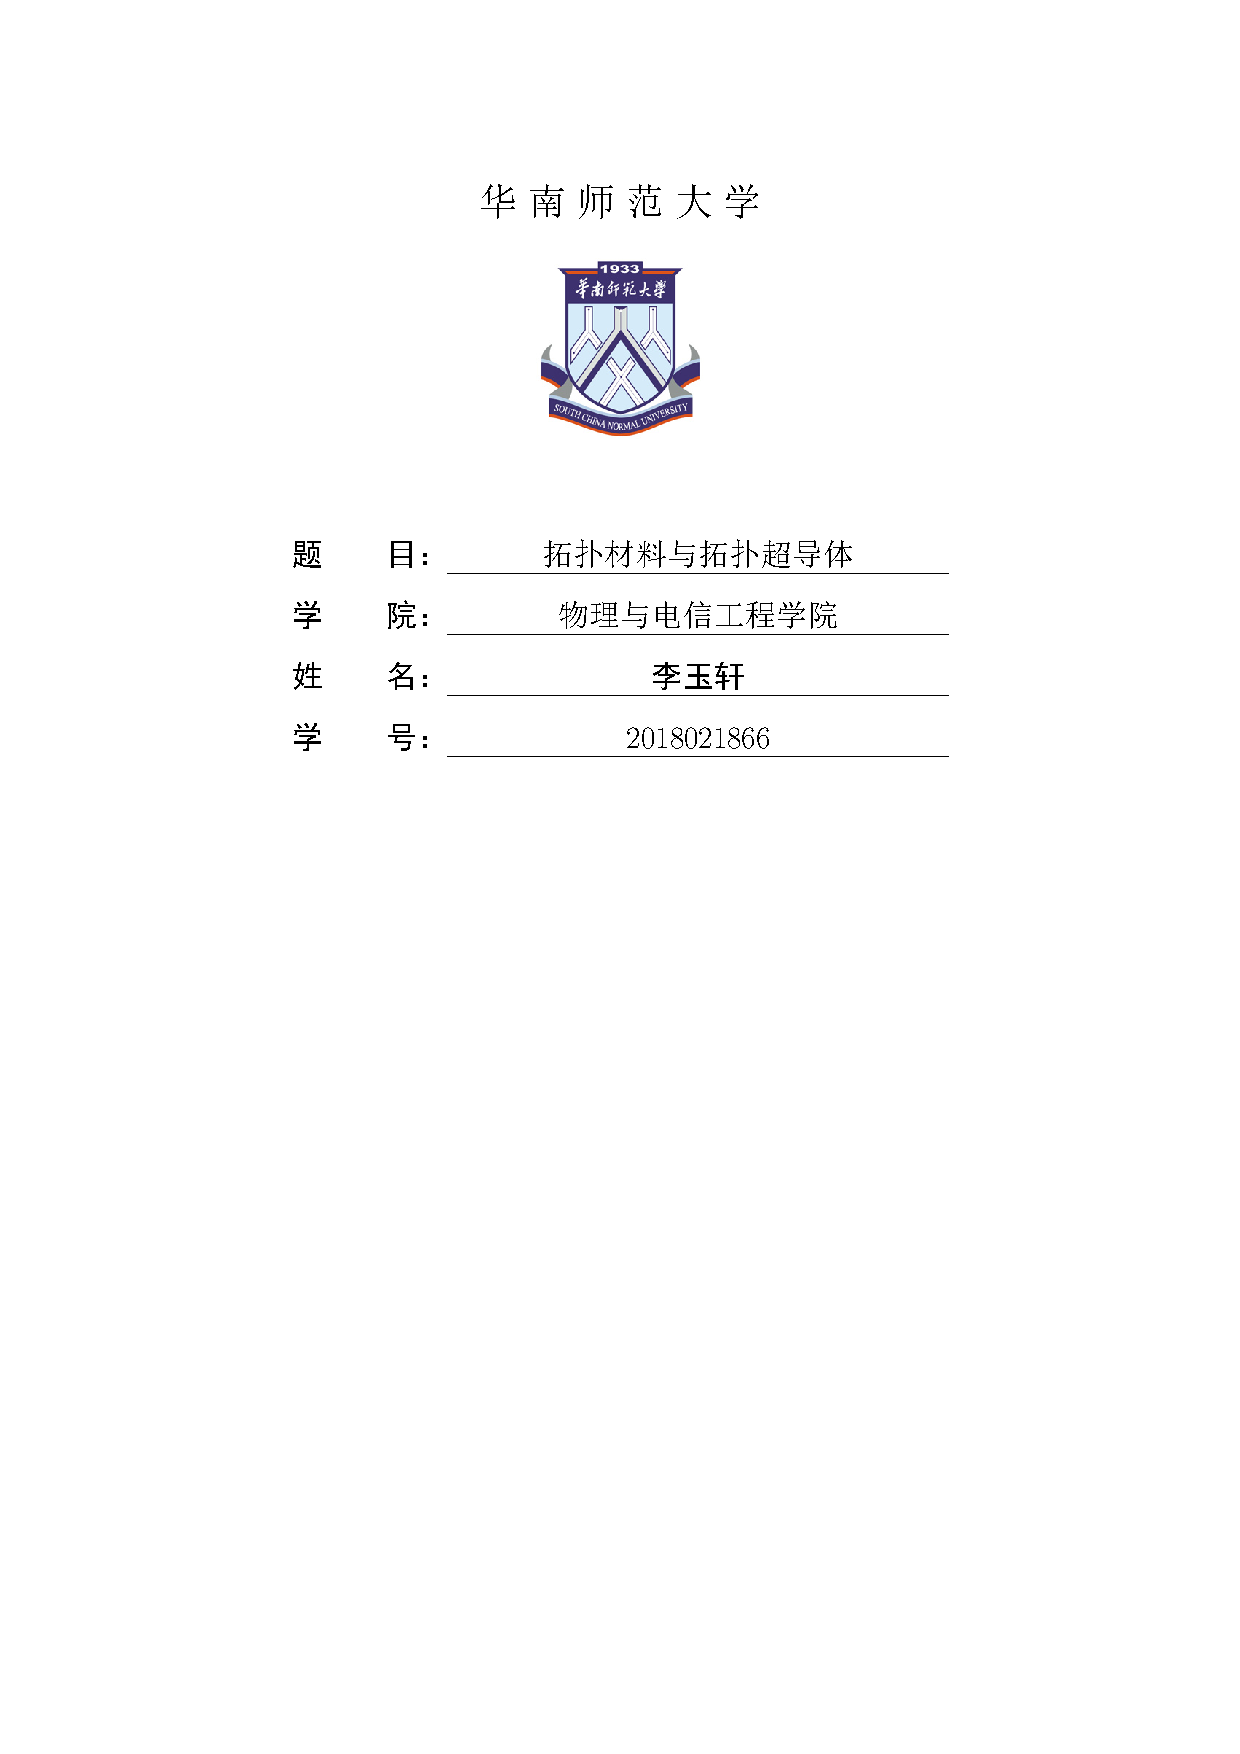
\includepdf{cover/cover.pdf}
\newpage
%\tableofcontents
\section{文档说明}
本手册用来记录在重复论文中遇到的问题,以及计算程序编写过程中,物理公式与程序语言之间的转换关系。本文档所有的代码均已上传至\href{https://github.com/yxli8023/BdG}{GitHub},在使用代码之前,请先阅读\textbf{ReadMe}文件,其中亦有作者的邮箱,欢迎讨论。
\section{模型建立}
代码是用来重复\href{https://github.com/yxli8023/BdG/blob/master/article/PhysRevB.96.184508.pdf}{Vortex pinning by the point potential in topological superconductors:A scheme for braiding Majorana bound states}中的数值结果,其中主要的模型内容如下所示:
\begin{equation}
H = H_t+H_{SO}+H_{SC}
\end{equation}
\begin{equation}
H_t = -\sum_{<ij>}t_0\Phi_{ij}(c_{i\sigma}^\dagger c_{j\sigma}+H.c)+\sum_{i\sigma}(\sigma h-\mu)c_{i\sigma}^\dagger c_{i\sigma}+\sum_\sigma V_ic_{i_0\sigma}^\dagger c_{i_0\sigma}
\end{equation}
\begin{equation}
H_{SO}=\sum_{i}(i\lambda\Phi_{ij} c_{i\uparrow}^\dagger c_{i+\hat{x}\downarrow}+i\lambda\Phi_{ij} c_{i\downarrow}^\dagger c_{i+\hat{x}\uparrow}+H.c.
+\lambda\Phi_{ij}c_{i\uparrow}^\dagger c_{i+\hat{y}\downarrow}
-\lambda\Phi_{ij}c_{i\downarrow}^\dagger c_{i+\hat{y}\uparrow}+H.c.)
\end{equation}
\begin{equation}
H_{SC}=\sum_i(\Delta_{ii}c_{i\uparrow}^\dagger c_{i\downarrow}^\dagger+H.c.)
\end{equation}
\begin{equation}
\sum_j 
\left[
\begin{array}{cccc}
H_{ij\uparrow\uparrow}&H_{ij\uparrow\downarrow}&\Delta_{jj}&0\\
H_{ij\downarrow\uparrow}&H_{ij\downarrow\downarrow}&0&-\Delta\\
\Delta_{jj}^\star&0&-H_{ij\downarrow\downarrow}^\star&-H_{ij\downarrow\uparrow}^\star\\
0&-\Delta_{jj}^\star&-H_{ij\uparrow\downarrow}^\star&-H_{ij\uparrow\uparrow}^\star
\end{array}
\right] \Psi_j^\eta=E_\eta\Psi_j^\eta\label{eq:5}
\end{equation}

where  $\Psi_j^\eta=(u_{j\uparrow}^\eta,u_{j\downarrow}^\eta,v_{j\downarrow}^\eta,v_{j\uparrow}^\eta)^T$and$\Delta_{jj}=\frac{V}{2}\sum_\eta u_{j\uparrow}^\eta v_{j\downarrow}^\eta\tanh(\frac{E_\eta}{2K_BT})$
$\sigma$代表自旋取向,向上为1向下为-1,$t_0$代表电子在相邻格点跳跃((hopping)时的能量,$\lambda$代表相邻格点之间的自旋轨道耦合(SOC)强度,$\Delta$是每个格点上不同自旋取向电子的配对能,$\mu$是体系的化学势,求和中的i是格点位置索引,公式中的i代表虚数单位。

通过模型建立,可以得到关于哈密顿量的矩阵形式,模型求解的关键点在于如何通过一系列的公式,正确的写出哈密顿量的矩阵形式,即就是方程(\ref{eq:5})中的矩阵。
\subsection{分析}
\begin{equation}
H=\sum_i(c_{i\uparrow}^\dagger,c_{i\downarrow}^\dagger,c_{i\downarrow},c_{i\uparrow}) \left[
\begin{array}{cccc}
H_{ij\uparrow\uparrow}&H_{ij\uparrow\downarrow}&\Delta_{jj}&0\\
H_{ij\downarrow\uparrow}&H_{ij\downarrow\downarrow}&0&-\Delta\\
\Delta_{jj}^\star&0&-H_{ij\downarrow\downarrow}^\star&-H_{ij\downarrow\uparrow}^\star\\
0&-\Delta_{jj}^\star&-H_{ij\uparrow\downarrow}^\star&-H_{ij\uparrow\uparrow}^\star
\end{array}
\right](c_{i\uparrow},c_{i\downarrow},c_{i\downarrow}^\dagger,c_{i\uparrow}^\dagger)^T
\end{equation}
\subsubsection{hopping项}
在模型求解过程中,主要是通过建立BdG方程,通过该方法可以实现矩阵的对角化,同时可以得到相应的本征值和本征矢量。从模型的建立来看,主要是通过紧束缚近似的离散晶格模型来构造哈密顿量,在紧束缚近似中,仅仅考虑了每个格点和相邻位置的跳跃和耦合,则可以明白\textbf{公式中的i和j仅仅代表的是最近邻格点位置},即就是$H_{i,j}$可能的形式为$H_{x,x\pm1}$和$H_{i,x\pm y}$,在将哈密顿量写成矩阵形式的过程中,可以清楚的看到hopping项是处于非对角线上的的位置,同时可以看到,最近邻位置之间跳跃时,自旋取向是相同的。
\subsubsection{couple项}
couple项的分析与hopping项分析过程类似,唯一不同的一点是,相邻格点之间的耦合,涉及到的是不同自旋取向之间的耦合,它的每一项仍然都处于矩阵的非对角线上。
\subsubsection{pair项}
从超导配对项的表达式中可以看到,它涉及到时同一个点不同自旋取向之间的配对,所以通过对矩阵的分析可以得知,它的每一项也都处于矩阵的非对角线上。
\subsubsection{others}
在hopping项中,第二项比较特殊($\sum_{i\sigma}(\sigma h-\mu)c_{i\sigma}^\dagger c_{i\sigma}$),从下角标可以知道,这一项同样是处于矩阵的对角线上,只不过不同的自旋取向对应着不同的值。自旋向上$\sigma=1$,自旋向下$\sigma=-1$,h代表的是Zeeman场的大小。
\subsection{矩阵构建}
假设我们考虑的晶格大小是xn*yn,通过分析过程可以得知对于hopping项($H_{ij\sigma\sigma}$),每个自旋取向$\sigma$对应的$H_{ij}$都是一个xn*yn的方阵
,根据方程(\ref{eq:5})中的矩阵形式,可以知道整个矩阵是一个行列都是xn*yn*4的矩阵。即通过模型,我们可以得到模型对应的矩阵是$H_{xn*yn*4,xn*yn*4}$。通过上面的分析,我们将整个矩阵分解为16个小矩阵,每个小矩阵的大小都是xn*yn,不过该矩阵的大多数元素都是0,属于稀疏矩阵。
在方程(\ref{eq:5})中,波函数$\Psi$的形式已经得知(即格点位置与自旋之间的联系),且注意到,索引指标j代表了晶格点阵的大小,j=xn*yn,前面已经将矩阵分解成了16个小矩阵,且其中又有4个都是零,则需要考虑填充的只有12个分块矩阵。
\subsection{hopping项矩阵填充}
hopping项中,不再对角线上的项是$c_{i\sigma}^\dagger c_{j\sigma}$,紧束缚近似仅考虑最近邻的格点之间的行为所以对于i格点上的电子,跳跃行为仅仅限于x+1(向右),x-1(向左),x+y(向上),x-y(向下),假定i格点在二维表示中为(a,b),且晶格大小为xn*yn,转换成矩阵元的时候它在矩阵元中的位置应该为(b-1)*yn+a*xn,令其等于m(m=(b-1)*yn+a*xn)
,它在矩阵中对角线上的位置为H(m,m),向右边的hopping在矩阵中的位置是H(m,m+1),向左边hopping即就是H(m,m-1),向上H(m,m+xn),向下H(m,m-xn)。以上的分析都只是对于(1,1)block进行的填充(方程\ref{eq:5}中的大矩阵在第一行第一列的小分块矩阵)。(2,2)block与(1,1)block之间的差别仅限于自旋取向的问题,不过在对(1,1)block和(2,2)block中的非对角线元素填充时,自旋的取向并不会影响元素的值,仅仅会影响hopping中对角线上元素的填充,在上一章节已经分析过,在此不做赘述。通过方程(\ref{eq:5})中矩阵的形式可以看到,(3,3)block和(4,4)block只不过是之前两个小分块矩阵的共轭,没有什么本质上的差别,其实将整个矩阵分解为16个小分块矩阵之后,对于相同物理效应,比如自旋轨道耦合,hopping,pari每个都对应4个分块矩阵,在矩阵填充的过程中,只需填充好一个,其余的三个就可以通过矩阵的平移变化得到。在跳跃过程中同时还会设计到波函数的位相问题,将在最后进行详细的讨论与说明。

下面将上述内容具体化:\\
(1,1)block:  ham(m,m+1)   ham(m,m-1)   ham(m,m+xn)   ham(m,m-xn)\\
(2,2)block: ham(xn*yn+m,xn*yn+m+1)   ham(xn*yn+m,xn*yn+m-1)   ham(xn*yn+m,xn*yn+m+xn)   ham(xn*yn+m,xn*yn+m-xn)\\
(3,3)block和(4,4)block的操作与上面的平移类似
\begin{figure}[h]
	\centering
	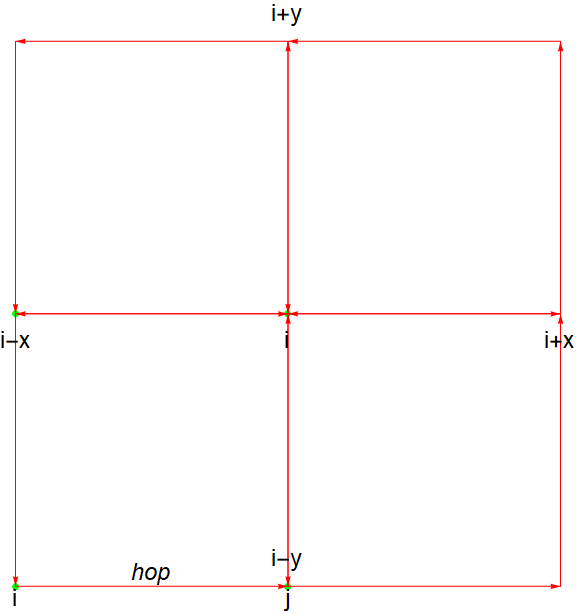
\includegraphics[scale=0.6]{lattice.png}
\end{figure}
\subsection{couple项矩阵填充}
couple项中,每一项都处于矩阵的非对角线上,填充的具体过程与hopping项方式一样,不过不同的一点在于,couple项在x和y方向上的填充值的形式是不同的,而hopping项中,不管是向那个方向进行跳跃,他的值的形式都是相同的,所以在对couple进行矩阵值填充是,需要格外注意这一点。\\
(2,1)block:  ham(m,xn*yn+m+1)   ham(m,xn*yn+m-1)   ham(m,xn*yn+m+xn) ham(m,xn*yn+m-xn)
\subsection{pari项矩阵填充}
(3,1)block:  ham(m,xn*yn*2+m+1)   ham(m,xn*yn*2+m-1)   ham(m,xn*yn*2+m+xn) ham(m,xn*yn*2+m-xn)

\section{矩阵填值分析}

\section{周期性边界问题}












\includepdf[pages=2]{file/prb.pdf}	
\end{document}